%!TEX root = ../main.tex
\section{Introduction}
\label{sec:intro}

\subsection{Context and the ``GT-free'' constraint}

Underwater, neither GPS nor cameras are usable in turbid water: the forward-looking
sonar (FLS) is often the only dense sensor. Bruce-SLAM~\hyperref[bib:bruceslam]{[1]} originally use IMU and DVL, but Aracati2017~\hyperref[bib:aracati]{[8]} has instead a direct command (\texttt{/cmd\_vel}) that is converted to an odometry.

The rule of this work is that \textbf{the final result must be obtainable on a real
UV}. The allowed sensors are the sonar, the on-board odometry and the USBL. The DGPS ground truth
(\texttt{/pose\_gt}) is forbidden — ground truth is
used for evaluation only. One documented nuance: the angular velocity of the
Aracati2017 on-board odometry is \emph{derived from the vehicle compass} (dataset
README~\hyperref[bib:aracati]{[8]}) — a compass is a legitimate on-board sensor; the consequence (near-exact
odometric heading, relative rotation error $\approx 0$) is the same as for the
``Odom+Mag'' baselines of DISO~\hyperref[bib:diso]{[3]} and ISOPoT~\hyperref[bib:isopot]{[4]}, and it is flagged wherever it
favours a metric.

\subsection{The Aracati2017 dataset}

Marina of Rio Grande (Brazil), LBV300-5 ROV navigating under a floating board
carrying a DGPS (\emph{position-only} ground truth — no orientation): 
\textbf{BlueView P900-130} sonar (130° field of view, 50 m range, Cartesian images),
velocity commands \texttt{/cmd\_vel}, USBL fixes \texttt{/usbl\_point}, compass.
A 44-minute mission ($\sim$1.5 km) along a T-shaped dock and pontoons (\autoref{fig:aracati}). The dataset is
known to be difficult (reflection artefacts, overexposed areas, cf.\ the ISOPoT
analysis~\hyperref[bib:isopot]{[4]}); DISO~\hyperref[bib:diso]{[3]} and ISOPoT~\hyperref[bib:isopot]{[4]} use it as a benchmark, which allows a
cross-reading of our numbers (\autoref{sec:protocole}).

\begin{figure}[H]
  \centering
  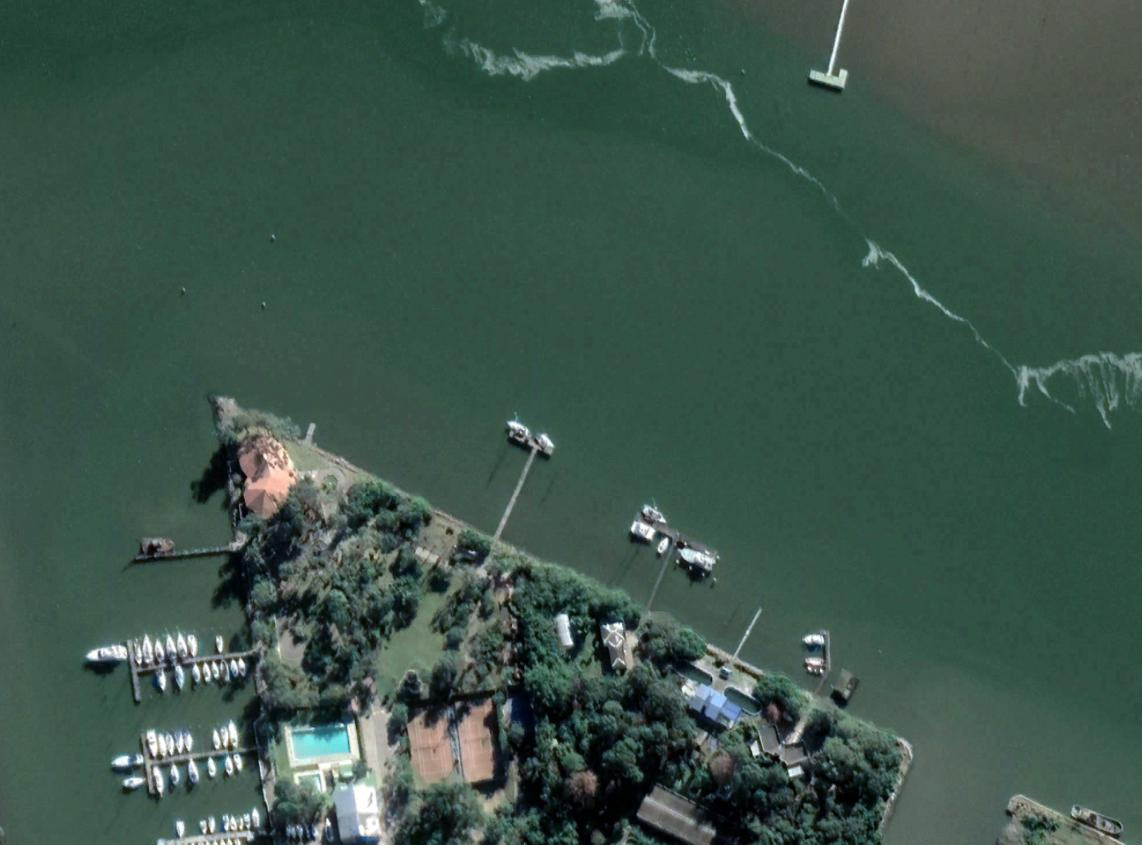
\includegraphics[width=0.8\textwidth, trim= 11cm 8cm 9cm 8cm, clip]{Image/aracati.png}
  \caption{Aracati2017 marina aerial view}
  \label{fig:aracati}
\end{figure}

\subsection{Pipeline}
\label{sec:pipeline}

\autoref{fig:pipeline} summarises the pipeline as actually executed, with the same
front-end / back-end split as the original Bruce-SLAM~\hyperref[bib:bruceslam]{[1]}:
the \textbf{front end} extracts the sonar features and computes the
\textbf{dead reckoning} that creates the keyframes and initialises the sequential
ICP; the \textbf{back end} is the iSAM2 factor graph, fed by the sequential
constraints, the verified loop closures and the USBL position factors. Chapter~1
(base method) covers the whole diagram with the native \emph{geometric} loop
detection of Bruce-SLAM; chapter~2 (proposed method) replaces \emph{only} the
candidate detection stage with appearance-based place recognition (Sonar Context
adapted to the P900) — the whole downstream geometric verification (shgo, ICP, PCM)
and the USBL anchoring are unchanged.

\begin{figure}[H]
\centering
\begin{tikzpicture}[
    font=\footnotesize,
    box/.style={draw=polytechblue, thick, rounded corners=2pt, fill=polytechblue!8,
                text width=3.0cm, align=center, minimum height=8mm, inner sep=3pt},
    sensor/.style={draw=black!60, thick, rounded corners=2pt, fill=black!5,
                text width=2.4cm, align=center, minimum height=8mm, inner sep=3pt},
    chap2/.style={draw=polytechlight, thick, rounded corners=2pt, fill=polytechlight!12,
                text width=3.0cm, align=center, minimum height=8mm, inner sep=3pt},
    outbox/.style={draw=polytechblue, very thick, rounded corners=2pt, fill=white,
                text width=2.6cm, align=center, minimum height=8mm, inner sep=3pt},
    fl/.style={-stealth, thick, draw=black!70},
    node distance=4mm and 7mm]

  % --- FRONT END : sonar chain (row 1) + dead reckoning (row 2)
  \node[sensor]            (sonar) at (0,0)     {P900 sonar\\ \tiny 130° polar images};
  \node[box]               (cfar)  at (3.6,0)   {SOCA-CFAR\\ detector};
  \node[box]               (chir)  at (7.2,0)   {Features\\ \tiny retained ``structure'' points};
  \node[box]               (kf)    at (10.9,0)  {Keyframes\\ \tiny displacement threshold, sequential ICP init.\ by the DR};
  \node[sensor]            (cmd)   at (0,-1.9)  {\texttt{/cmd\_vel}\\ \tiny $v_x$ on-board, $\omega_z$ compass};
  \node[box]               (unic)  at (3.6,-1.9) {Dead reckoning\\ \tiny unicycle $\theta_{k+1}{=}\theta_k{+}\omega_z\Delta t$};
  \node[draw=black!50, dashed, thick, inner sep=2.5mm, rounded corners=2pt,
        fit=(sonar)(cfar)(chir)(kf)(cmd)(unic),
        label={[black!60, font=\footnotesize\itshape]north west:front end}] (fe) {};

  % --- BACK END : loop detection + verification + factor graph + USBL factors
  \node[box]               (nssm)  at (5.4,-4.3) {\textbf{Chap.~1}: candidates by proximity / covariance};
  \node[chap2]             (sc)    at (5.4,-5.9) {\textbf{Chap.~2}: Sonar Context adapted to the P900\\ \tiny density descriptor + Polar Key kNN + 10 m gate};
  \node[box, text width=2.4cm] (verif) at (9.2,-5.1) {Verification:\\ shgo $\to$ ICP $\to$ PCM};
  \node[box, text width=2.5cm, fill=polytechblue!15] (graph) at (9.2,-7.7)
       {\textbf{iSAM2 factor graph}};
  \node[box]               (cauchy) at (3.6,-7.7) {Robust unary factor (Cauchy)\\ \tiny temporal association to KF, position only};
  \node[sensor]            (usbl)  at (0,-9.6)  {USBL\\ \tiny noisy position fixes};
  \node[draw=black!50, dashed, thick, inner sep=2.5mm, rounded corners=2pt,
        fit=(nssm)(sc)(verif)(graph)(cauchy),
        label={[black!60, font=\footnotesize\itshape]south west:back end}] (be) {};

  % --- outputs
  \node[outbox] (traj)  at (13.4,-9.6) {2D trajectory};
  \node[outbox] (carte) at (9.2,-9.9) {Map (point cloud)};

  % --- flows
  \draw[fl] (sonar) -- (cfar);
  \draw[fl] (cfar) -- (chir);
  \draw[fl] (chir) -- (kf);
  \draw[fl] (cmd) -- (unic);
  \draw[fl] (unic.east) -| ($(kf.south)+(-4mm,0)$);
  \draw[fl] (usbl.east) -| (cauchy.south);
  \draw[fl] ($(kf.south)+(4mm,0)$) |- (nssm.east);
  \draw[fl] ($(kf.south)+(4mm,0)$) |- (sc.east);
  \draw[fl] (nssm.south) |- ($(verif.west)+(0,2mm)$);
  \draw[fl] (sc.east) -- ++(4mm,0) |- ($(verif.west)+(0,-2mm)$);
  \draw[fl] (verif.south) -- (graph.north);
  \draw[fl] (kf.east) -- ++(4mm,0) |- ($(graph.east)+(4mm,1mm)$) -- ($(graph.east)+(0,1mm)$);
  \draw[fl] (cauchy.east) -- ($(graph.west)+(0,0)$);
  \draw[fl] ($(graph.east)+(0,-1mm)$) -- ++(4mm,0) |- (traj.west);
  \draw[fl] (graph.south) -- (carte.north);
\end{tikzpicture}
\caption{Pipeline as actually executed, front-end / back-end split of the original
system. Grey: allowed on-board sensors (never the ground truth). Dark blue: common
pipeline (chapter~1). Light blue: the only stage replaced in chapter~2
(appearance-based loop candidate detection). The sequential factors of the graph
are the dead-reckoning deltas between keyframes. The USBL acts in the back end
only (robust position factors); its two possible front-end roles — seeding the
frame at $t_0$ (used in chapter~1) and continuously correcting the dead reckoning
(complementary filter) — are kept out: enabling the front-end correction together
with the back-end factors is a contradictory double anchoring (measured $\times$3
ATE degradation, \autoref{sec:usbl}).}
\label{fig:pipeline}
\end{figure}

\subsection{Evaluation protocol: origin-anchored comparison}
\label{sec:protocole}

All the numbers in this document use the \textbf{origin-anchored} comparison (also
called ``first pose''): it is the convention of the published tables on Aracati
(DISO~\hyperref[bib:diso]{[3]}, ISOPoT~\hyperref[bib:isopot]{[4]}) and the most realistic one — every method starts
from the same known point, and the metric accumulates the actual drift from this
start instead of spreading it with an optimal a posteriori fit (Umeyama-style).

\paragraph{a) Start-pinned ATE.} The estimated trajectory and the ground truth are
both translated so that they start at $(0,0)$. \emph{No rotation is fitted, on
anything}: the orientation of the estimated frame is part of the system output. In
the final configuration it is initialised at a fixed zero heading, the GT-free
equivalent of the \texttt{/initialpose} a deployed vehicle receives. We validated
this rule offline before adopting it:
\begin{itemize}
\item a rigid fit of the integrated odometry onto the DGPS track over the first
  10--30 m puts the true initial heading within 1--2.5° of zero, and the same fit
  onto the USBL track does no better (2--4°);
\item a naive course-over-ground seed would be off by 45--78° even on a 30 m
  baseline: the vehicle turns by 88° during its first 30 m, so the course is not
  the heading. Earlier runs that seed from the first USBL fixes (position +
  course-over-ground) are labelled as such where they appear.
\end{itemize}
The ATE is the RMSE of the point-to-point distances
(temporal association). Two properties of this rule:
\begin{itemize}
\item it has \emph{zero free parameter} and is identical for every method, run and
  section — nothing from the ground truth enters the estimate, not even an
  orientation anchor;
\item it is \emph{stricter} than the published protocol: ISOPoT~\hyperref[bib:isopot]{[4]} re-anchors each
  section with the magnetometer heading, we never re-fit any orientation. As a
  sanity check, our odometry evaluated in a fixed-heading frame gives
  \textbf{6.00 / 12.62 / 8.44 m} per section, close to the
  \textbf{5.8 / 12.5 / 6.5 m} of the ``odometry alone'' row published by ISOPoT on
  the same data (\autoref{sec:compare}).
\end{itemize}

\paragraph{b) Sections S1/S2/S3.} DISO evaluates Aracati as 3 sequences of
$\sim$15 min (odometry restarted at each section); the exact boundaries are not
published. We split the continuous mission into \textbf{temporal thirds}, each
section being \textbf{re-pinned in translation at its own start} (no rotation, same
rule as §a). Two consequences to keep in mind:
\begin{itemize}
\item a section carries the frame-heading error accumulated up to its start — our
  sections are \emph{not} given a fresh orientation, unlike the published ones;
\item our SLAM methods close loops \emph{across} sections (an advantage), while the
  published odometries restart from zero (a disadvantage) — the cross-reading is
  indicative, not a ranking.
\end{itemize}

\paragraph{c) Relative errors (RE), comparable to the DISO/ISOPoT tables.} For each
start index $i$, take the ground-truth track segment of length $L$ = 10~\% of the
section, and compare the relative displacements expressed in the frame of pose $i$:
\begin{equation}
e_{\text{trans}} = \frac{100}{|S|} \sum_{i}
\frac{\lVert \Delta\hat{\mathbf{p}}_i - \Delta\mathbf{p}_i \rVert}{L_i}\ [\%],
\qquad
e_{\text{rot}} = \frac{1}{|S|} \sum_{i}
\frac{|\Delta\hat\theta_i - \Delta\theta_i|}{L_i}\ [°/\text{m}]
\end{equation}
This is the metric least sensitive to anchoring conventions, hence the most
comparable across papers. The ground-truth heading $\theta$ comes from the compass —
reliable on this dataset (emerged sensor~\hyperref[bib:isopot]{[4]}), but \emph{identical} to the source of
$\omega_z$: the rotation error of every ``Odom+Mag'' method (ours included) is
$\approx 0$ by construction, and the meaningful comparison is on translation.

\paragraph{d) Heading error over time.} The estimated heading $\theta_k$ and the
compass heading $g_k$ (NED) differ by a convention: we fit
$g_k \approx s\,\theta_k + \beta$ ($s = \pm 1$, $\beta$ = circular mean of the
residual), then report the wrapped residual — median and RMS. The removed offset
$\beta$ is a frame choice, not an error of the method.

\paragraph{e) Map error.} The usual point-cloud metrics (self-consistency) measure
\emph{sharpness}, not \emph{correctness}. We re-render \textbf{the same detections}
at the ground-truth poses: each point is brought back into the local frame of its
keyframe through the estimated pose, then re-projected through the ground-truth pose
(DGPS position, compass heading $s\,(g_k - \beta)$ — never DISO nor any third-party
method). The map error of a point is its distance to the nearest neighbour in this
``true cloud''; we report the median and the 90\textsuperscript{th} percentile. With
identical detections, this metric isolates the map degradation caused by pose errors
alone.

The whole protocol is implemented in \texttt{analysis/paper\_eval.py} and
\texttt{analysis/paper\_figs\_origine.py}; the numbers and figures of this document
come directly from them.

\subsection{Contributions and outline}

\begin{enumerate}
\item \textbf{GT-free odometric chain}: unicycle integration of the \texttt{/cmd\_vel}
  commands + robust unary USBL factors (Cauchy kernel) in the iSAM2 factor graph
  (\autoref{sec:chap1}).
\item \textbf{Appearance-based loop detection}: Sonar Context~\hyperref[bib:sonarcontext]{[2]} re-derived for the
  low-resolution P900 (density descriptor instead of max-pooling,
  AUC 0.55 $\to$ 0.86), with a geometric gate and a documented threshold calibration
  (\autoref{sec:chap2}).
\item \textbf{Explicit evaluation protocol} (start-pinned, zero fit, per section;
  RE; map metric) and \textbf{controlled comparison} with the published methods on
  this dataset: start-pinned ATE of \textbf{1.94--2.00 m} over the 44 min mission,
  relative translation error of \textbf{5.0~\%} against 9.69~\% for the best
  published assisted method (ISOPoT), and better values than every published method
  on \emph{all three} sections (chapter~2, \autoref{sec:compare}).
\end{enumerate}

Chapter~1 presents the base method (Bruce-SLAM adapted GT-free) and its results;
chapter~2 the proposed method (Sonar Context + USBL) and the full comparison.
Chapter~3 validates the approach in the HoloOcean simulator and extends the map
to 3D with two additional sonars, the base pipeline kept unchanged.
